% Template for IGARSS-2020 paper; to be used with:
%          spconf.sty  - LaTeX style file, and
%          IEEEbib.bst - IEEE bibliography style file.
% --------------------------------------------------------------------------
\documentclass{article}
\usepackage{spconf,amsmath,epsfig}
\usepackage{bm,bbm}
\usepackage{float}
\usepackage{epstopdf} %para imagenes en eps y 
%%%
\usepackage{url}
\usepackage{booktabs,chemformula}
\addtolength{\tabcolsep}{-0.3em}
%\usepackage[backend=biber,style=phys,doi=false,eprint=false,url=false]{biblatex}
%\usepackage{booktabs, longtable,array}
%\usepackage[table]{xcolor}
%\newcolumntype{P}[1]{>{\raggedright\arraybackslash}p{#1}}
%\usepackage[a4paper,margin=1in]{geometry}
%%%
%\addbibresource{\jobname.bib}
% \newcommand{\mcite}[1]{\mbox{\cite{#1}}}

% Example definitions.
% --------------------
\def\x{{\mathbf x}}
\def\L{{\cal L}}

\DeclareMathOperator{\Tr}{Tr}

%


% Title.
% ------
\title{Quality assessment measures for explainable fusion of statistical evidences of edges in PolSAR images: A First Approach}
% Single address.
% ---------------

%\address{Author Affiliation(s)}
\name{Rosa Janeth Alpala$^a$, Anderson A.\ de Borba$^{b,c}$, and Alejandro C.\ Frery$^c$.\thanks{e-mail:$^{a}$janeth.alpala@ufpe.br,$^{b}$anderson.borba@mackenzie.br, $^c$alejandro.frery@vuw.ac.nz}}
\address{$^a$ Universidade Federal de Pernambuco, 50740-540, Recife, PE, Brazil,           \\
$^b$Mackenzie Presbyterian University--UPM, FCI, BigMAAp, SP -- Brazil, \\
$^c$School of Mathematics and Statistics, Victoria University of Wellington, 6140, New Zealand.}

%
\begin{document}
%\ninept
%
\maketitle
%
\begin{abstract}
\vspace{-0.2cm}
This work aims to develop techniques for the fusion of statistical evidences obtained from the application of Statistical Information Theory (SIT) and Statistical Information Geometry (SIG) in image processing and analysis, with a specific focus on Polarimetric Synthetic Aperture Radar (PolSAR) imagery. The goal is to generate a single solution superior to individual solutions. Furthermore, properties or measures that assess the quality of results will also be employed to evaluate the effectiveness of fusion methods in detecting edge evidence.

%
\begin{keywords}
PolSAR, edge detection,  information fusion,  quality
measures 
\end{keywords}
%
\end{abstract}
\vspace{-0.3cm}
\section{Introduction}
\vspace{-0.2cm}
PolSAR images offer a distinct advantage over other remote sensing images by utilizing four different polarization combinations, specifically HH, HV, VH, and VV~\cite{Hua2022}. These combinations are based on the horizontal (H), and vertical (V) polarizations of the received and transmitted signals. 
 
Edge detection in PolSAR images plays an essential role in many applications, such as speckle noise reduction, superpixel segmentation, land-cover classification, and target recognition~\cite{Jin2016}. 


The study by de Borba et al.~\cite{DeBorba2020} is the foundation for this research. 
It finds evidence of the location of edge points by using a deterministic approach that does not take into account the variability of the estimator. We extended this research by incorporating several quality metrics that not only assess the accuracy of the edge estimate, but also provide insight into the explainability of the fused edge evidence.
%We extended this investigation using various quality metrics to evaluate and compare the results of fusing edge evidence in PolSAR images.

The remaining of this paper is organized as follows: Section \ref{sec_2} provides a brief introduction to the background knowledge, including PolSAR data and edge detection. Section 3 presents an overview of the quality measures employed. The evaluation of edge estimation quality using various metrics is discussed in Section 4. Lastly, conclusion is provided in Section 5.


\section{Background}\label{sec_2}
\vspace{-0.2cm}
\subsection{PolSAR data representation}
Using PolSAR data, a wide range of biophysical and geophysical parameters related to the Earth's surface can be efficiently and reliably extracted. The polarimetric scattering matrix~\cite{Lee2017} serves as an instrumental tool to represent the polarimetric target information:
\begin{equation}
 \mathbf{S} = \begin{bmatrix}
S_{\text{HH}} & S_{\text{HV}} \\
S_{\text{VH}} & S_{\text{VV}}
\end{bmatrix},  
\label{E:a1}
\end{equation}
where the elements $S_{\text{HH}}$ and $S_{\text{VV}}$ are the returned power in the co-polarized channels, while the elements $S_{\text{HV}}$ and $S_{\text{VH}}$ relate to the cross-polarized channels.
If the PolSAR targets comply with the reciprocal condition $(S_{\text{HV}} = S_{\text{VH}})$, single-look PolSAR data can be represented using a scattering vector:
\begin{equation}
\mathbf{k}_s=[S_{\text{HH}}, \sqrt{2}S_{\text{HV}}, S_{\text{VV}} ]^t,
\label{E:21}
\end{equation}
where  the superscript $t$ stands for the transpose operation. 
Multi‑look PolSAR data can be expressed  by a covariance matrix  given as 
\(\mathbf{C}=\langle\mathbf{k}_S\mathbf{k}_S^\text{H} \rangle= {L}^{-1} \sum_{i=1}^{L} \mathbf{k}_s(i)\mathbf{k}_s(i)^\text{H} \), where $\langle \cdot \rangle$ is the ensemble average, $\text{H}$  the is complex conjugate transpose operator, and $L$ is the number of looks. 
The covariance matrix is hermitian, i.e., $\mathbf{C}= \mathbf{C}^\text{H}$, and positive definite;
see Ref.~\cite{Qin2022}.

\subsection{Gamma distribution}
%Over the past decades, several distributions have been created for modeling PolSAR image data. The most commonly used distribution for working with images generated from polarimetric multilook data is the complex Wishart distribution~\cite{Nielsen2007}. This distribution is characterized by two parameters, the covariance matrix $\mathbf{\Sigma}$ and the number of looks L of the image. Thus, the polarimetric matrix $\mathbf{Z} = \mathbf{C}=\left\langle\mathbf{k}_s\mathbf{k}_s^H \right\rangle$ can be derived following a complex Wishart distribution, represented as $\mathbf{Z}\sim \mathcal{W}_{\mathcal{C}}(\mathbf{\Sigma}, L),$  whose probability density function
%is~\cite{Frery2014, Qin2022}:
%\begin{align}
%f_{\mathbf{Z}}(\mathbf{Z})=\frac{L^{qL}|\mathbf{Z}|^{L-q}}{|\mathbf{\Sigma}|^L\Gamma_q(L)}\exp\left\{-L \Tr\left(\mathbf{\Sigma}^{-1}\mathbf{Z}\right)\right\},
%\label{E:22}
%\end{align}
%where $\Gamma_q(L)=\pi^{q(q-1)/2}\prod_{i=0}^{q-1}\Gamma(L-i)$,  $\Gamma(\cdot)$ denotes the gamma function and $\Tr(\cdot)$ is the trace of the matrix. In this case, three channels will be used, i.e., $q = 3$.

We assume that the distribution of each intensity channel  follows a Gamma law, characterized by the probability density function
\begin{equation}
f_Z(z;\mu,L)=\frac{L^{L}z^{L-1}}{\mu^{L}\Gamma(L)} \exp\big\{-Lz/\mu\big\},\quad z>0,
\label{func_dens_uni_gamma}
\end{equation}
where $L>0$, and
$\mu>0$ is the mean.
The log-likelihood of the sample $\bm{z} = (z_1,\dots,z_n)$ under this model is
\begin{equation}
\mathcal{L}(\mu, L; \bm{z}) = 
n \big[L\ln (L / \mu) - \ln \Gamma(L)\big]
+L \sum_{k=1}^{n}\ln z_k -\frac{L}{\mu}\sum_{k=1}^{n} z_k.
\label{eq:LogLikelihoodGamma}
\end{equation}
Then, we find $\big(\widehat \mu, \widehat L\big)$, the maximum likelihood estimator (MLE) of $(\mu, L)$ from $\bm{z}$, by maximizing~\eqref{eq:LogLikelihoodGamma}.

% A simplified derivation to obtain the complex Wishart distribution was presented in \cite{LEE1994}.
\subsection{Edge detection on a single data strip}
Finding the edges of an image is a crucial step in image analysis. These boundaries define distinct regions within the image, such as pastures, urban areas, or forested areas~\cite{monferran2020modelo}. Various techniques, including maximum likelihood, entropy, and geodesic distance, are commonly used in research studies to identify edge points~\cite{NaranjoTorres2017,Nascimento2019}. 
Suitable statistical models are needed for locating edge points in these types of images.

The Gambini algorithm~\cite{Gambini2007} is a highly appealing method for edge detection. 
It searches for evidence of edges within a narrow data strip. 
The algorithm involves projecting rays and identifying edge evidence by maximizing a value function.

The algorithm starts by casting rays from a point inside the candidate region, e.g., the centroid.
Data are collected around each ray to form the sample $\bm z = (z_1,z_2,\dots,z_n)$, which is partitioned at position $j$ into the interior $\bm z_\text{I}$ and exterior $\bm z_\text{E}$ samples:
$$
\bm z = (\underbrace{z_1,z_2,\dots,z_j}_{\bm z_\text{I}}, 
\underbrace{z_{j+1}, z_{j+2},\dots,z_n}_{\bm z_\text{E}}).
$$
Two possibly different models are assumed for each partition:
$\bm Z_\text{I} \sim \Gamma(\mu_\text{I},L_\text{I})$, and 
$\bm Z_\text{E} \sim \Gamma(\mu_\text{E},L_\text{E})$.
We then estimate $(\mu_\text{I},L_\text{I})$ and $(\mu_\text{E},L_\text{E})$ with $\bm z_\text{I}$ and $\bm z_\text{E}$, respectively, by maximizing~\eqref{eq:LogLikelihoodGamma}, and obtain $\big(\widehat{\mu}_\text{I}, \widehat{L}_\text{I}\big)$ and $\big(\widehat{\mu}_\text{E}, \widehat{L}_\text{E}\big)$.

Then, the total log-likelihood is
\begin{equation}\label{eq:TotalLogLikelihood}
\begin{aligned}
\mathcal L\big(j&;\widehat{\mu}_I, \widehat{L}_I,\widehat{\mu}_E, \widehat{L}_E\big)= -\Bigg(
	\frac{\widehat{L}_\text{I}}{\widehat{\mu}_\text{I}}\sum_{k=1}^{j} z_k +
	\frac{\widehat{L}_\text{E}}{\widehat{\mu}_\text{E}}\sum_{k=j+1}^{n} z_k  
	\Bigg)\mbox{}\\
&+j \big[\widehat{L}_\text{I}\ln (\widehat{L}_\text{I} / \widehat{\mu}_\text{I}) - \ln \Gamma(\widehat{L}_\text{I})\big]
+\widehat{L}_\text{I} \sum_{k=1}^{j}\ln z_k  \mbox{}\\
&+(n-j) \big[\widehat{L}_\text{E}\ln (\widehat{L}_\text{E} / \widehat{\mu}_\text{E}) - \ln \Gamma(\widehat{L}_\text{E})\big]
+\widehat{L}_\text{E} \sum_{k=j+1}^{n}\ln z_k .%-\\ 
\raisetag{2.2em}
\end{aligned}
\end{equation}
The estimate of the edge position on the ray is the coordinate  $\widehat\jmath$ which maximizes $\mathcal L$.
\vspace{-0.2cm}
\subsection{Fusion methods for edge evidence}
De Borba et al.~\cite{DeBorba2020} fused the edges evidence obtained in intensities channels HH, HV, and VV to produce a unique and more accurate edge position estimator. 
The authors used six fusion methods: simple average, multiresolution discrete wavelet transform (MRDWT), principal component analysis (PCA), receiver operating characteristic (ROC) statistics, multiresolution stationary wavelet transform (MR-SWT), and a multiresolution method based on singular value decomposition (MR-SVD).

Edge evidence fusion methods are essential to quantify and qualify the information obtained from each image channel. 
Such information enables the decision to utilize or discard data from a specific channel to enhance edge detection accuracy.

\section{Quality assessment}
\vspace{-0.2cm}
Commonly used quality measures for performance evaluation include Mean Absolute Error (MAE) and Root Mean Square Error (RMSE). MAE calculates the average absolute difference between estimated and reference values, being robust against outliers and independent of error signs. In contrast, RMSE emphasizes larger errors, making it more sensitive to outliers \cite{Ritter2013}. Additional precision evaluation measures include Standard Deviation (SD) and Correlation Coefficient (CC). SD measures the dispersion of values relative to their average, higher SD indicates lower precision. CC quantifies the linear relationship between the value sets~\cite{Vijayaraj}. The formulas are as follows:
\begin{align*}
	\text{RMSE} =\sqrt{\frac{1}{n}\sum_{i=1}^{n}\left(y_i-\hat{y}_i\right)^2},
	%\label{rmse}
\end{align*}
\vspace{-0.3cm}
\begin{align*}
	\text{MAE} =\frac{1}{n}\sum_{i=1}^{n}|y_i-\hat{y}_i|,
	%\label{mae}
\end{align*}
\begin{align*}
	\text{SD} =\sqrt{\frac{1}{n-1}\sum_{i=1}^{n}\left(y_i-\bar{y}\right)^2},
	%\label{sd}
\end{align*}
\begin{align*}
\text{CC}=  \frac{\sum_{i=1}^{n}(x_i-\Bar{x})(y_i-\Bar{y})}{\sqrt{\sum_{i=1}^{n}(x_i-\Bar{x})^2\sum_{i=1}^{n}(y_i-\Bar{y})^2}},
%\label{cc}
\end{align*}
where $n$ represents the number of observations, $y_i$ denotes the estimated values, $\hat{y}_i$ are the reference measured values, and  $\Bar{x}$ and $\Bar{y}$ are the mean values.

 Another metric that is used is the entropy, this quantifies the uncertainty of a probability distribution. In information theory, it reflects the level of uncertainty in a random experiment or signal. A peaked distribution has low entropy and low uncertainty, while a homogeneous distribution has high entropy and high uncertainty \cite{Mays2002}. For a discrete random variable $X$ with $\left\{x_1, x_2, \ldots, x_N\right\}$ the set of possible values it can take, Shannon entropy is defined as:
\begin{align}
	H(X)=-\sum_{i=1}^{N}p(x_i)\log_2p(x_i),
	\label{eq:H}
\end{align}
where $p(x_i)$ represents the probability of $i$th element in the vector.

Entropy is commonly used in remote sensing to describe the information content of images. It employs expression \eqref{eq:H}  to assess the amount of information conveyed by each pixel within an image. 

\vspace{-0.2cm}
\section{RESULTS}
\vspace{-0.2cm}
Figs.~\ref{fig:res}(a)-(c) show the edge evidences in the HH, HV and VV channels obtained through maximum likelihood estimation.
De Borba et al.~\cite{DeBorba2020} applied various fusion methods to detect edge evidence. 
As an example, the results obtained by applying PCA, ROC and MR-SWT methods to an AIRSAR L-band image of Flevoland are shown in Fig.~\ref{fig:fus}.%(a)-(b).



\begin{figure}[H]
   % \centering
    \begin{minipage}{0.5\textwidth}
       \begin{minipage}[b]{.32\linewidth}
  \centering
 \centerline{\epsfig{figure=figures/hh_f.pdf,width=2.8cm}}
  \vspace{-0.1cm}
  \centerline{\small{(a) Channel HH.}}\medskip
\end{minipage}
\begin{minipage}[b]{.31\linewidth}
  \centering
\centerline{\epsfig{figure=figures/hv.pdf,width=2.8cm}}
  \vspace{-0.1cm}
  \centerline{\small{(b) Channel HV.}}\medskip
\end{minipage}
%\hfill
\begin{minipage}[b]{0.31\linewidth}
  \centering
 \centerline{\epsfig{figure=figures/vv_c.pdf,width=2.8cm}}
  \vspace{-0.1cm}
  \centerline{\small{(c) Channel VV.}}\medskip
\end{minipage}\vspace{-0.3cm}
       \caption{Edges evidences from the three intensity channels.}
\label{fig:res}
    \end{minipage}%\hfill
\end{figure}
\vspace{-0.4cm}
\begin{figure}[H]
   % \centering
    \begin{minipage}{0.5\textwidth}
       \begin{minipage}[b]{.32\linewidth}
  \centering
 \centerline{\epsfig{figure=figures/roc.pdf,width=2.75cm}}
  \vspace{-0.1cm}
  \centerline{\small{(a) ROC fusion.}}\medskip
\end{minipage}
\begin{minipage}[b]{.31\linewidth}
  \centering
\centerline{\epsfig{figure=figures/pca_1.pdf,width=2.8cm}}
  \vspace{-0.1cm}
  \centerline{\small{(b) PCA fusion.}}\medskip
\end{minipage}
%\hfill
\begin{minipage}[b]{0.31\linewidth}
  %\centering
 \centerline{\epsfig{figure=figures/swt.pdf,width=2.75cm}}
  \vspace{-0.1cm}
  \centerline{\small{(c) MR-SWT fusion.}}\medskip
\end{minipage}\vspace{-0.3cm}
       \caption{Fusion methods.}
\label{fig:fus}
    \end{minipage}%\hfill
\end{figure}\vspace{-0.2cm}

Figs.~\ref{fig:entropy1}(a)-(c), illustrate the total log-likelihood $\mathcal L$ functions with respect to the $j$th position, where these functions exhibit peaks that potentially serve as indicators of edge position. Specifically, the concept of entropy is used as a means of evaluating the accuracy of edge position.\vspace{-0.3cm}
\begin{figure}[H]
   % \centering
    \begin{minipage}{0.5\textwidth}
       \begin{minipage}[b]{.5\linewidth}
  \centering
 \centerline{\epsfig{figure=figures/likelihood_hh.pdf,width=5cm}}
  \vspace{-0.1cm}
  \centerline{\footnotesize{ (a) Channel HH (\textbf{Entropy = 0.0546}).}}\medskip
\end{minipage}%\hfill
\begin{minipage}[b]{.5\linewidth}
  \centering
\centerline{\epsfig{figure=figures/likelihood_hv.pdf,width=5cm}}
  \vspace{-0.2cm}
  \centerline{\footnotesize{(b) Channel HV (\textbf{Entropy =  0.6361}).}}\medskip
\end{minipage}\\
\hfill 
\vspace{-0.3cm}
 \centering
\begin{minipage}[b]{0.5\linewidth}
  \centering
 \centerline{\epsfig{figure=figures/likelihood_vv.pdf,width=5cm}}
  \vspace{-0.1cm}
  \centerline{\footnotesize{(c) \, Channel VV  (\textbf{Entropy =  0.8577}).}}\medskip
\end{minipage}\vspace{-0.2cm}
       \caption{Entropy as a quality measure for edge evidence.} 
\label{fig:entropy1}
    \end{minipage}%\hfill
\end{figure}
\vspace{-0.3cm}
To calculate entropy,  we employ the transformation of the total log-likelihood function, into a discrete probability function, the sample is taken from a single data strip (ray) of length 120 pixels.  Subsequently, expression~\eqref{eq:H} is used to calculate the Shannon entropy, $H(X)$. The resulting value provides an objective metric for evaluating the accuracy of edge point detection. A low entropy value signifies precise estimation, characterized by a compact and peaked curve, see Fig.~\ref{fig:entropy1}(a). Conversely, a high entropy value suggests less accurate estimation, featuring a more dispersed probability distribution and a graph with a flatter and elongated shape, see Fig.~\ref{fig:entropy1}(b)-(c).\par
%\vspace{-0.1cm}
On the other hand, the aim of this study is to determine whether evidence fusion in PolSAR images provides more information, leading to accurate edge detection, compared to edge detection of individual channels.\par
%\vspace{-0.1cm}
Table~\ref{tab_1} illustrates the evaluation metrics employed to assess the quality of the estimated edge points by comparing their similarity with a predefined set of reference points. These metrics offer an objective evaluation of the accuracy of the obtained results. Entropy is calculated exclusively using the estimated edge point dataset ($\hat{x},\hat{y}$), while the remaining metrics (MAE, RMSE, SD, and CC) utilize both datasets. 
\begin{table}[H]
  \centering
  \begin{tabular}{@{}cccccc@{}}
    \toprule
Method  &Entropy    & MAE        & RMSE       &SD       & CC \\
    \midrule
   hh  & 6.6439      & 1.8400       & 3.7175   & 2.6291   & 0.9986 \\
   hv  & 6.6293      & 1.6700       & 2.9275   & 2.0640   & 0.9992 \\
   vv  & 6.6438      & 4.2400      & 7.9461    & 5.5649   & 0.9941 \\
   ROC & 6.0223      & 1.4154      & 2.3664    & 1.6311    & 0.9994 \\
   PCA & 7.7944      & 3.0180       & 6.0657   & 4.2788  & 0.9964 \\
   SWT & 12.0914     & 5.8006      & 9.2486   & 6.4161  & 0.9932 \\
    \bottomrule
  \end{tabular}\vspace{-0.1cm}
  \caption{\small{Assessment metrics.}}
  \label{tab_1}
\end{table}\vspace{-0.3cm}
The importance of entropy calculation is highlighted. For instance, with the ROC method, we observe low error and high correlation, indicating significant similarity between edge point positions. However, the low entropy value suggests a relatively small amount of information in the fused image. This implies precise edge detection with few outliers, but exhibiting a sparse distribution of points, as shown in Fig.~\ref{F4}. \vspace{-0.45cm}
\begin{figure}[H] %\vspace{-2.0mm} 
	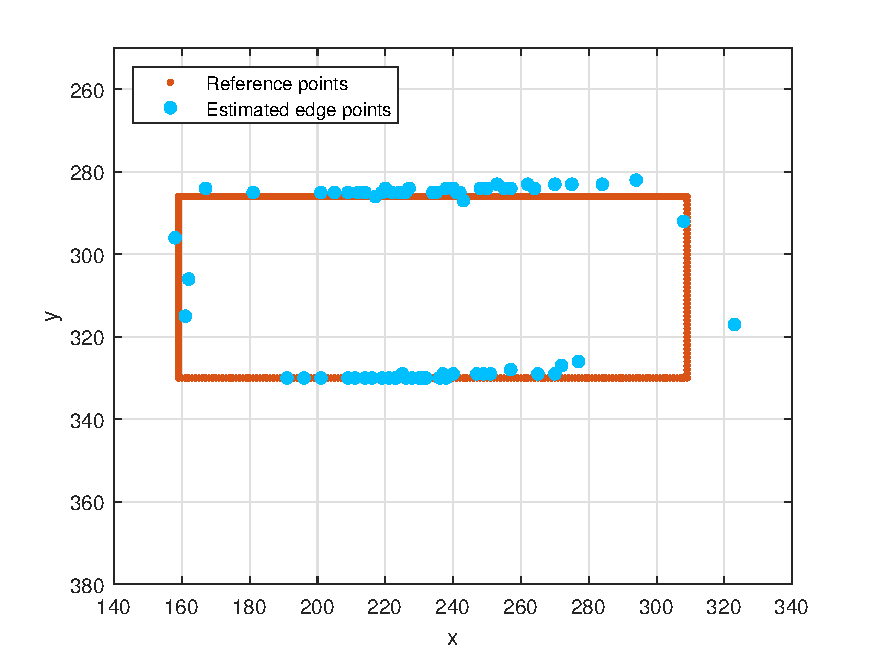
\includegraphics[scale=0.55]{figures/roc_f.pdf}\vspace{-1.5mm} 
	\caption{Comparison of estimated points with reference points.}
	\label{F4}
\end{figure}
On the other hand, the PCA method demonstrates superior performance, as it exhibits a moderate entropy value along with low values of MAE, RMSE, and SD.

This approach enables a comprehensive evaluation of the characteristics and performance of fusion methods and individual channels. All metrics are depicted in Fig.~\ref{F5}. \vspace{-0.3cm}
\begin{figure}[H] 
	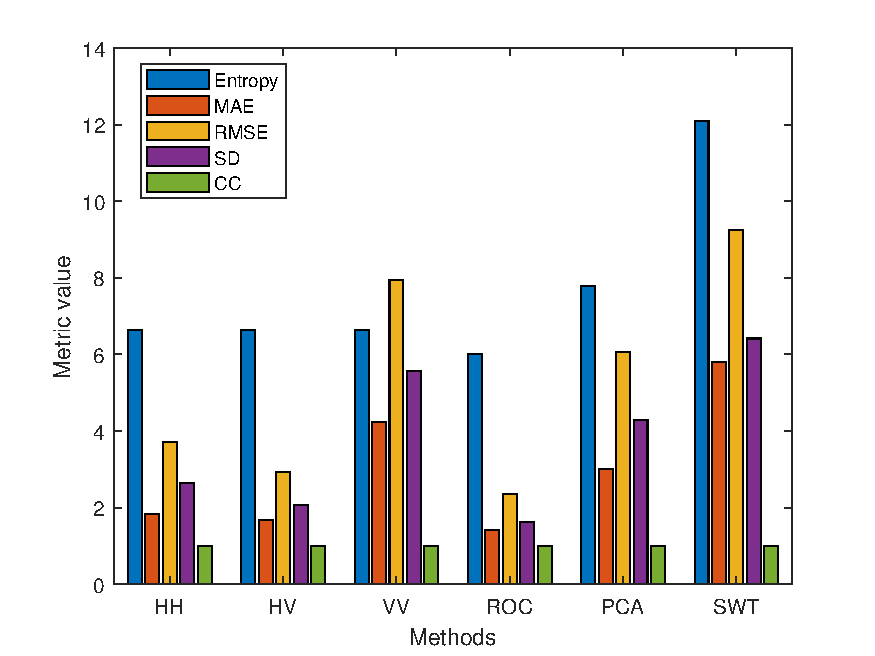
\includegraphics[scale=0.55]{figures/metricas.pdf}\vspace{-3.5mm} 
	\caption{illustration of quality metrics.}\vspace{-0.3cm}
	\label{F5}
\end{figure}%\vspace{-0.1cm}
The method for detecting edge evidence  and fusion methods were implemented in Python. Code and data are available for download at:  \url{ https://github.com/rjaneth/code_igarss_23.git}
\vspace{-0.3cm}
\section{CONCLUSION}
\vspace{-0.3cm}
This paper presents some fusion methods for edge evidence and assesses their estimation precision using commonly employed metrics in the literature, with a specific emphasis on entropy as the primary measure.

By incorporating entropy as an evaluation metric, we enhance the explainability of our fusion methodology. Entropy provides a quantitative measure of the diversity and variability of the detected edges, allowing us to assess the amount of information captured by the fusion process. This transparency in evaluating the results enhances the interpretability and trustworthiness of our approach.

Overall, the results demonstrate the effectiveness of the proposed fusion methods for edge evidence and highlight the importance of incorporating explainability measures, such as entropy, in the evaluation process. These findings contribute to the field of image and data fusion, providing insights into the information content and accuracy of the detected edges.


% References should be produced using the bibtex program from suitable
% BiBTeX files (here: strings, refs, manuals). The IEEEbib.bst bibliography
% style file from IEEE produces unsorted bibliography list.
% ------------------------------------------------------------------------
%\bibliographystyle{IEEEtranS}
%\bibliographystyle{IEEEbib-abbrev}
\bibliographystyle{IEEEtran}
%\bibliography{strings,refs}

\bibliography{../../Common/references}
\end{document}
